%
%
%% Section: USE CASES
%%\section{Clouds in Community Networks}
%%\label{sec:use-cases}
%
%%Since our community cloud is targeted to be used in real community networks, it is a must that our architecture, design, implementation and deployment fits into these conditions and scenarios. 
%%We focus our analysis on the Guifi.net community network, which is considered the largest community network worldwide, and it is where we have also deployed our prototype.
%%
%\subsection{Community Networks}
%
%%%%%%%%%%%%%%%%%%%%%%%%%%%%%%%%%%%%%%%%%
%\subsubsection{Nodes and topological aspects of community networks}
%
%A community network is managed and owned by the community, where nodes are managed independently by their owners. 
%The computer machines or nodes in a community network vary widely in their capacity, function and capability, as illustrated in Figure~\ref{fig:community-network}.
%Some hardware is used as super nodes (SN) that have multiple wireless links and connect with other SNs to form the backbone of the community network, and are usually intended to be stable with permanent connectivity.
%Most SNs are installed in the community network participant's premises. 
%A few SNs, however are placed strategically in a third party location, e.g. telecommunication installations of municipalities, to improve the community network's backbone.
%Other nodes in the community network act as ordinary nodes (ON) and are only connected to the access point of a SN. 
%Topological analysis of the Guifi.net community network~\cite{Vega2012} indicates that from approximately 17,000 analysed nodes of Guifi.net, 7\% are SNs while the others are ONs.
%
%From the node types shown in Figure~\ref{fig:community-network}, it can be seen that 
%principally the hardware for computation and storage is already available in community networks, consisting of some servers attached to the networking nodes. 
%No cloud services, however, are yet deployed in community networks to use this hardware as a cloud, leaving the community network services significantly behind the current standard of the Internet. 
%Our vision is that some community wireless routers will have cloud resources attached, building the infrastructure for a community cloud formed by several cloud resources attached to the nodes. 
%We note that ONs could principally also contribute cloud resources.
%
%
%Figure~\ref{fig:outdoor_node} shows the outdoor view of a community network SN. 
%The equipment, mainly antennas and radios, is used for building wireless links between other SNs. 
%Figure~\ref{fig:SN_Real} shows an example of the indoor hardware of a SN. 
%The router used is a Microtik RB750, while a Jetway JBC362F36W with Intel Atom N2600 CPU, 2GB RAM and 64GB USB has been added to become a cloud resource for the community cloud.
%A laptop is used as an additional server, while a UPS keeps the node running in the case of power failure.
%
%\begin{figure}[tbp]
%	\centering
%	\begin{minipage}[c]{0.45\linewidth}
%		\centering
%		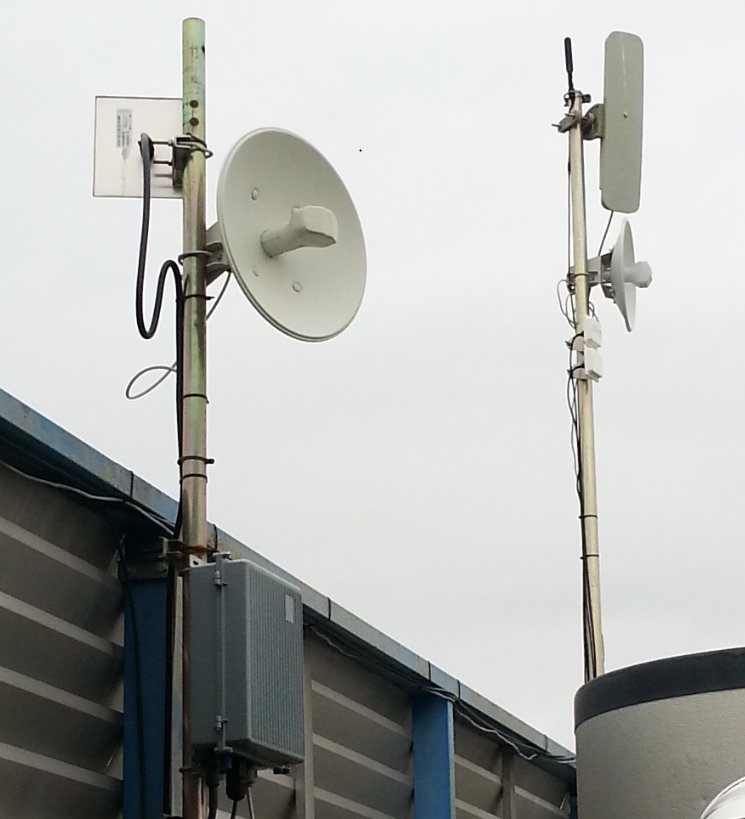
\includegraphics[width=2.55in,keepaspectratio]{outdoor_node2}
%		\caption{SN with outdoor hardware for wireless links}
%		\label{fig:outdoor_node}
%	\end{minipage}
%	\quad
%	\begin{minipage}[c]{0.45\linewidth}
%		\centering
%		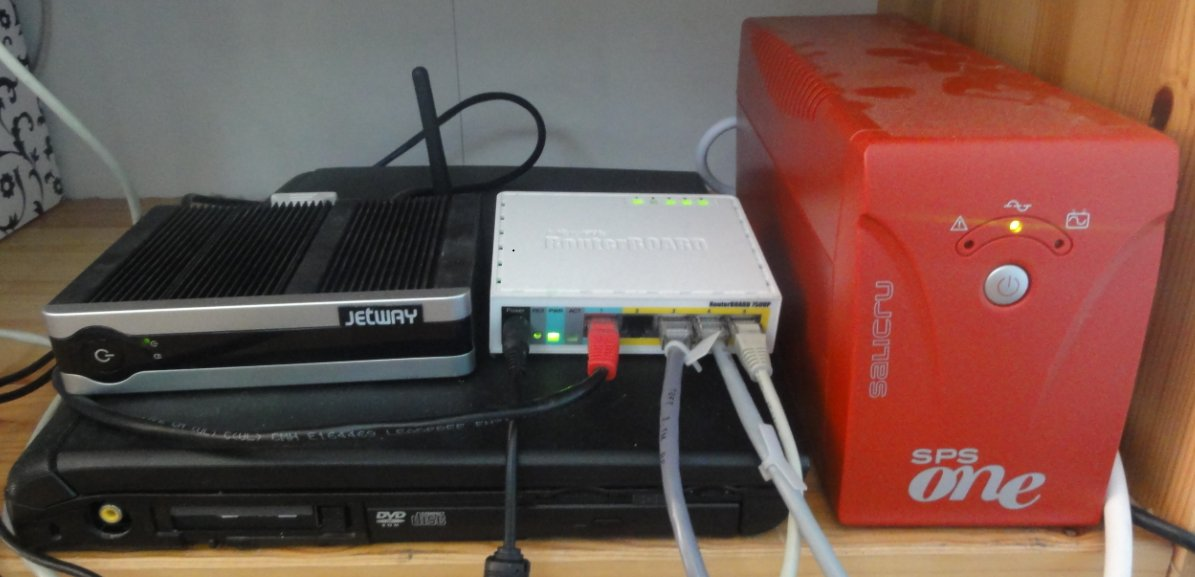
\includegraphics[width=2in,keepaspectratio]{SN_Real}
%		\caption{Indoor hardware of a community network node with router, server and cloud resource}
%		\label{fig:SN_Real}
%		%		
%		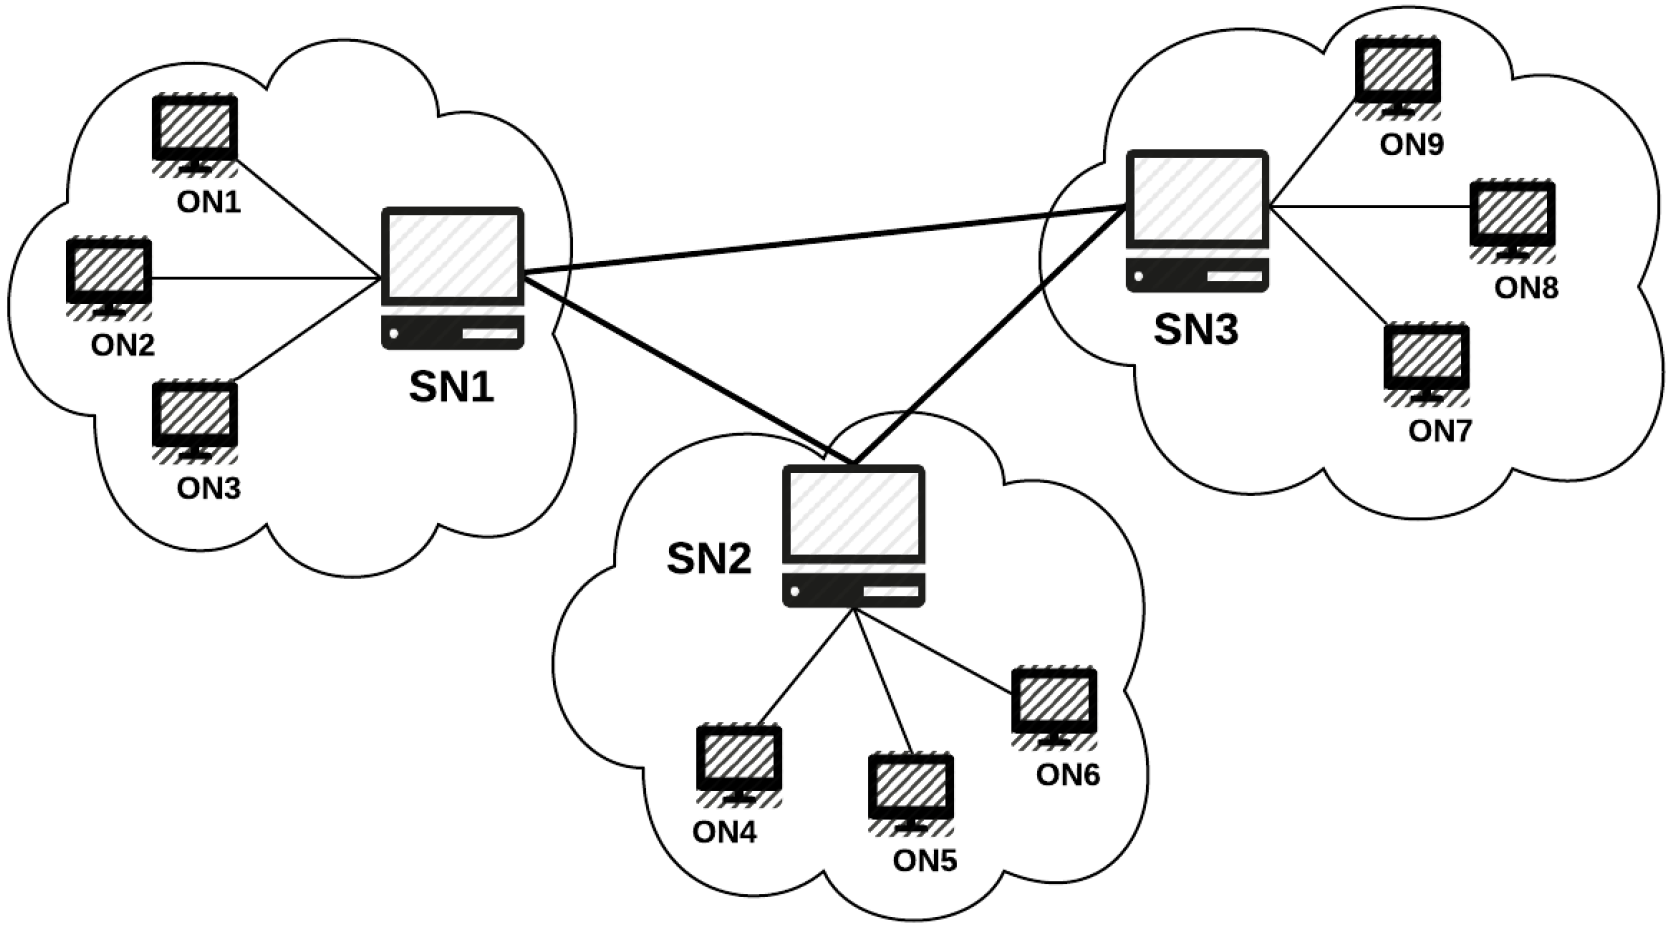
\includegraphics[width=2.4in,keepaspectratio]{federated_cloud}
%		\caption{Nodes in federated community cloud}
%		\label{fig:federated_cloud}
%	\end{minipage}	
%\end{figure}
%
%%%%%%%%%%%%%%%%%%%%%%%%%%%%%%%%%%%%%%%%%
%\subsubsection{Social aspects of community networks}
%
%Personal and social relationships play an important role in the community network deployment. 
%The deployment of new nodes requires the collaboration among people. 
%If a new node is deployed, the owners of the neighbouring nodes need to connect with it, thus there has to be an interaction among the people. 
%Two types of social networks can be observed from Guifi.net's mailing list~\cite{GuifinetForum}. 
%One is at the global level of the whole Guifi.net network. 
%In this list, technical issues are discussed. 
%People from any part of Guifi.net community participate, and even external people who are interested can take part. 
%The second type is the local social network, between node owners within a zone and between neighbouring zones. 
%They use local mailing lists as well as hold weekly meetings.
%
%Guifi.net is organised into zones. 
%A zone can be a village, a small city, a region, or a district of a larger city. 
%The organization of the group within a zone is of many types. 
%Mostly the interests, available time and education of the people drive what happens in the zone. 
%We note that while the allocation of IP addresses and layer 3 networking is agreed among all Guifi.net zones, as it is needed to make the IP network work, the detailed technical support is rather given within the local community of the zone. 
%Therefore, we identify a zone to have the highest social strength within the community network.
%
%%%%%%%%%%%%%%%%%%%%%%%%%%%%%%%%%%%%%%%%%
%\subsubsection{Members of community networks}
%
%Participants of community networks are principally consumers and producers of the network. 
%Most of them as producers contribute infrastructure and time to the networks, while as consumers they use the available services the network offers. 
%The community network, however, is not maintained solely based on the contribution of infrastructure. 
%Some users must also contribute with their time and knowledge.
%Time is needed, for instance, for maintenance tasks, which might require technical knowledge or not. 
%Technical knowledge is required because the network is an IP network, which needs to be managed and configured. 
%
%%%%%%%%%%%%%%%%%%%%%%%%%%%%%%%%%%%%%%%%%
%\subsubsection{Resource sharing in community networks}
%
%Community networks are a successful case of resource sharing among a collective. 
%The resources shared are networking hardware but also community network participants' time that they donate, to different extent, for maintaining the network. 
%While the community network infrastructure is the sum of the individual contributions of wireless equipment, the network operation is achieved by the contribution of time and knowledge of the participants.
%This is because even under the decentralised management of the equipment, the owner of the device ultimately has the full access and control of that network device.
%
%Reciprocal resource sharing is, in fact, part of the membership rules or peering agreements of many community networks. 
%The Wireless Commons License (WCL)~\cite{WCL2010} of many community networks states that the network participants that extend the network, e.g. contribute new nodes, will extend the network in the same WCL terms and conditions, allowing traffic of other members to transit on their own network segments.
%Therefore, resource sharing in community networks from the equipment perspective refers in practice to the sharing of the nodes' bandwidth. 
%This sharing, done in a reciprocal manner, enables the traffic from other nodes to be routed over the nodes of different node owners and allows community networks to successfully operate as IP networks. 
%We observe that in most community networks the focus at the moment is on the bandwidth sharing alone.
%There is not much awareness about sharing other computing resources, such as storage or CPU time, inside of community networks. 
%
%
%%%%%%%%%%%%%%%%%%%%%%%%%%%%%%%%%%%%%%%%%
%\subsubsection{Ownership of nodes in community networks}
%
%Community networks grow organically. 
%Typically a new member that wants to connect to the community network contributes with the hardware required to connect to other nodes. 
%A node of a community network therefore belongs to the member who is its sole owner. 
%Such a node is normally located in the member's premises. 
%
%Although less typical, a few nodes in Guifi.net have also been successfully crowd-funded if such a node was needed by several people. 
%Crowd-funding of a node happened when for a group of people an infrastructure improvement was necessary. 
%For example, an isolated zone of Guifi.net established a super node to connect to other zones. 
%In such a case, the node has been purchased with the contributions of many people. 
%The location of such a node follows strategic considerations, trying to optimise the positive effects on the performance that are achieved with the addition of the new infrastructure.
%We can see that both the options, individual ownership and crowd-funding of resources, occur in practice and could be considered for community clouds.
%
%%%%%%%%%%%%%%%%%%%%%%%%%%%%%%%%%%%%%%%%%
%\subsubsection{Services in community networks} 
%
%Services and applications offered in community networks usually run on the machines that the member connects to the network and these machines are used exclusively by that member. 
%The usage of the community network's services among its members, beyond that of access to the Internet, is however not very strong.
%
%\subsection{Community Cloud Scenarios}
%Based on the socio-technical characteristics of community networks analysed above, we start sketching our vision of community clouds.
%
%%%%%%%%%%%%%%%%%%%%%%%%%%%%%%%%%%%%%%%%%
%\subsubsection{Local Community Cloud}
%
%This scenario is derived from the topology of the community network, given by the fact that 
%the community network generally has two different types of nodes, SNs and ONs, 
%and the observed characteristics of the strength of social network within zones~\cite{Vega2012}. 
%In such a local community cloud, a SN is responsible for the management of a set of attached nodes contributing cloud resources. 
%From the perspective of the attached nodes, this SN acts as a centralised unit to manage the cloud services. 
%
%%%%%%%%%%%%%%%%%%%%%%%%%%%%%%%%%%%%%%%%%
%\subsubsection{Federated Community Cloud}
%
%Multiple SNs from different zones in a community network can connect and form federated community cloud~\cite{Moreno-Vozmediano2012}.
%SNs connect physically with other SNs through wireless links and logically in an overlay network to other SNs that manage local clouds.
%SNs coordinate among themselves for provisioning infrastructure service so the requests originating from one SN's zone can be satisfied by the resources allocated from another SN's zone.
%Figure~\ref{fig:federated_cloud} shows an example of a federated community cloud formed by SNs from three zones.
%The ONs in a given zone are directly managed by the SN in that zone but they can also consume resources from other zones because of the coordination among SNs.
